\providecommand{\StudySection}{\section}
\providecommand{\StudySubsection}{\subsection}

\StudySection{Learning from complete reduction time}
\label{sec:workflow}
The scattering test shows why a useful equation label is an incomplete training objective for acceleration. A filter can retain sufficient equations and still add more overhead than it saves. We therefore train a model to predict complete reduction time and let it choose the initial seed region, an optional seed or equation filter, and an integral ordering. The model makes one choice for the whole target batch before Kira begins its exact calculation.

To evaluate that choice fairly, we also need a baseline with the same surrounding implementation. We combine the earlier equation filter with an existing improvement in temporary data handling, which reduces execution cost without changing the equations or arithmetic. The \emph{integrated native control} uses this implementation with Kira's own decisions. Comparing the learned strategy with that control measures the benefit of the prediction beyond the shared implementation changes.

For a target batch, let $B=(r_{\max},s_{\max},q_{\max})$ contain the largest positive index sum, numerator rank, and dot count. A dot is one denominator power above one. Table~\ref{tab:workflow-actions} lists the strategies considered, and Appendix~\ref{app:workflow} defines the quantities and derives the cost models. The seed limits and ordering options are provided by Kira~\cite{Kira12}; ordering five changes the priority of sectors while retaining the within-sector preference of ordering one. All strategies must return the same prescribed master basis.

\begin{table}[!htbp]
\centering\small
\caption{Strategies available to the complete-time model. Negative seed
bounds are replaced by zero. Native row choices remain active.}
\label{tab:workflow-actions}
\begin{tabular}{@{}ll@{}}\toprule
Strategy & Initial seed region and selection\\\midrule
Integrated native & Bounds $B$; native choices\\
Smaller region & Bounds $B-(1,1,1)$; native choices\\
Fewer dots & Bounds $B-(1,0,1)$; native choices\\
Equation filter & Bounds $B$; saved equation tree\\
Seed filter & Bounds $B$; saved seed tree where available\\
Different ordering & Bounds $B$; Kira ordering five\\
Larger region & Bounds $B+(1,1,1)$; native choices\\\bottomrule
\end{tabular}
\end{table}

A smaller region can avoid unnecessary equation generation, while a larger region can avoid a failed first attempt when the target's own index limits are insufficient. If the initial strategy fails the basis check, the calculation tries native choices at $B$ and then at $B+(1,1,1)$ when needed. The native control also enlarges an insufficient region, and every failed attempt contributes to the training and test time. For the four earlier multiloop graphs, the seed-filter option uses native choices because this implementation has no separate seed tree for them. Its equation-filter option uses the earlier trees for those graphs and the newly trained trees for the three additional scattering structures.

The model receives eighteen features describing the graph, symbolic variables, number of targets, index powers, and sectors. For each strategy, its training label is the logarithm of the complete-time ratio to integrated native choices. We compare a constant predictor, six regression trees, three ridge-regression models, and two nearest-neighbour models. Regression trees follow the squared-error construction of Ref.~\cite{CART1984}; Appendix~\ref{app:workflow} specifies all candidates. Validation selects ridge regression with penalty $\lambda=10$ and decision margin $\gamma=0$, giving validation ratio $0.993$.

The best fixed strategy selected from training is integrated native reduction. Consequently, the integrated-native and best-fixed controls use the same settings in independent trials, and differences between their times indicate execution variation. The seed and equation trees retain their earlier weights throughout this study, and learned row selection remains disabled.

The data contain 31 training batches, 17 validation batches, and 31 test batches from the sunrise, planar box, three-loop vacuum, three-loop ladder, nonplanar box, pentagon, and box with external virtuality. Rational batches use different masses or invariants across the splits, while additional symbolic batches use different target lists. These are new inputs within seven known graph structures at one through three loops. The recurrence study through twelve loops remains a separate result for its restricted vacuum family.

Each training and validation cost uses three repetitions. Testing uses five repetitions to compare the preceding native implementation, integrated native choices, the best fixed strategy, and the learned strategy. The controller and models are loaded before timing, but every attempt starts a fresh Kira process. Timers include input preparation, prediction, native IBP generation, algebra, exact checks, cleanup, and retries. They exclude training, enlarged reference reductions, and later recording of results. Additional application checks measure cold startup and compare returned coefficients after a reduction supplied only with its targets and basis. For an unknown graph or target complexity outside the training range, the learned application uses native choices; the same guard applies to combined requests.

\StudySubsection{Results for individual target batches}
All 620 timed calculations pass exact checks of 59,640 coefficient entries, and all 31 applications supplied without reference coefficients pass their subsequent comparisons. Each timed method makes fifteen fallback attempts. Thus this model changes some initial strategies but does not remove the remaining cases that need a second attempt.

Relative to the preceding native implementation, the learned strategy has time ratio $0.9903$, with descriptive interval $[0.9796,0.9996]$, or about 1.0\% less time. Its ratio to integrated native choices is $0.9965$ with interval $[0.9875,1.0070]$, and its ratio to the best-fixed control is $1.0026$ with interval $[0.9979,1.0081]$. Both comparisons with the matched integrated controls include equal time. They therefore provide no reliable additional saving from the learned choices. The two identically configured controls have ratios $0.9938$ and $0.9878$ to the preceding native implementation, illustrating the scale of execution variation.

Table~\ref{tab:workflow-times} reports the results by graph. The aggregate averages logarithmic ratios within each graph and then gives all seven graphs equal weight, as derived in Appendix~\ref{app:workflow}. The smallest learned-to-native ratio is $0.9654$ for the three-loop vacuum, while the ladder and nonplanar box take slightly more time. These results motivate testing more specific strategies for each graph rather than enabling the common model for all inputs.

\begin{table}[!htbp]
\centering\small
\caption{Complete-cost results. Native seconds are geometric means of
batch median times. The other entries are geometric mean time ratios;
a value below one means less time.}
\label{tab:workflow-times}
\begin{tabular}{@{}lrrrr@{}}\toprule
Graph & Native (s) & Integrated/native & Learned/native & Learned/integrated\\\midrule
Sunrise & 0.502 & 1.0123 & 0.9932 & 0.9811\\
Planar box & 1.621 & 0.9906 & 0.9771 & 0.9864\\
Three-loop vacuum & 0.726 & 0.9745 & 0.9654 & 0.9907\\
Three-loop ladder & 3.535 & 1.0146 & 1.0013 & 0.9869\\
Nonplanar box & 3.119 & 1.0075 & 1.0073 & 0.9998\\
Pentagon & 0.599 & 0.9758 & 0.9942 & 1.0189\\
Box with virtuality & 0.484 & 0.9824 & 0.9944 & 1.0122\\
\bottomrule
\end{tabular}
\end{table}

\begin{figure}[!htbp]
\centering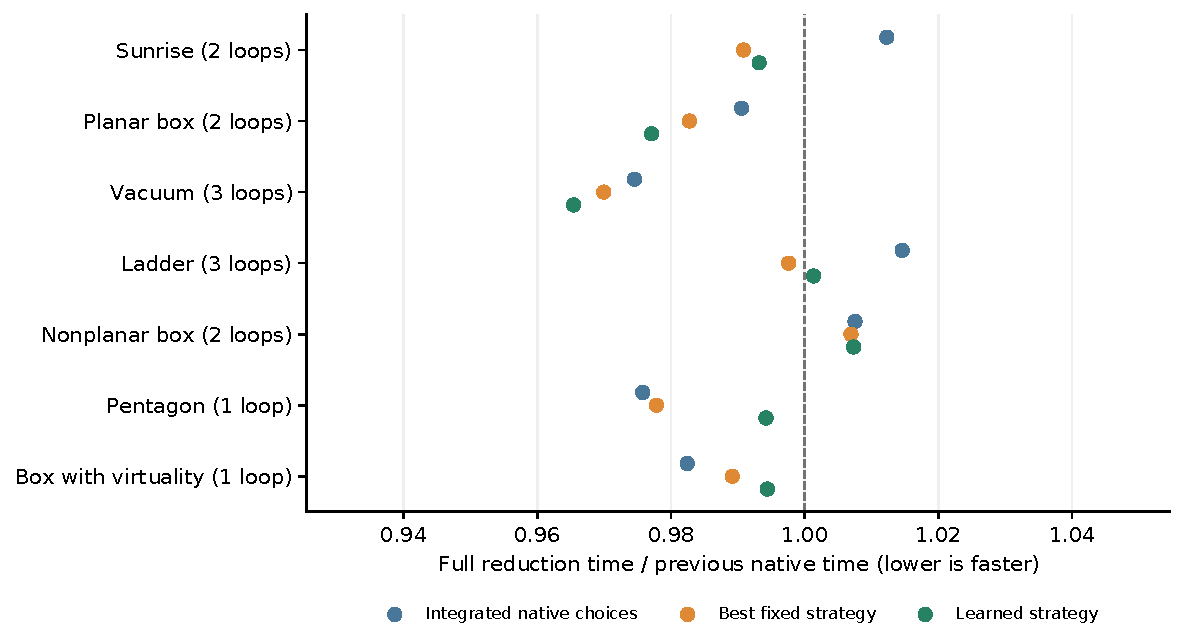
\includegraphics[width=\linewidth]{paper_figures/workflow_time.pdf}
\caption{Learned choices and the native controls have similar complete times.
The best-fixed and integrated controls use the same configuration in
separate trials. The plot shows variation across graph structures;
the text gives the aggregate uncertainty intervals. The axis focuses
on the measured range and retains the equal-time line.}
\label{fig:workflow}
\end{figure}

\FloatBarrier

\StudySubsection{Sharing a reduction between compatible requests}
Before changing the predictor, we test whether repeated work can be removed from the way Kira receives targets. When two available requests have the same family and kinematics, their target lists can be combined and reduced together. The resulting coefficient rows are then returned to the appropriate request. This shares family preparation and algebra between the lists. Appendix~\ref{app:workflow} defines the ten request groups and derives this separation from linearity; the model and its settings remain fixed.

Five repetitions of four methods give 200 complete calculations, all of which pass exact checks. Joint native reduction has ratio $0.5252$ to two separate native reductions. With the integrated implementation and native choices, the ratio is $0.5175$ with interval $[0.5073,0.5346]$, giving 48.3\% less time or speedup $1.93$ with interval $[1.87,1.97]$. Every tested graph group benefits from the shared reduction. Its integrated-native ratios range from $0.5040$ to $0.5679$, corresponding to savings of 43.2--49.6\%.

The joint learned strategy has ratio $0.5152$ to separate native requests, but its ratio to joint integrated native choices is $0.9955$ with interval $[0.9810,1.0058]$. As Table~\ref{tab:joint} and Figure~\ref{fig:joint} show, the main gain comes from sharing the calculation; the predictor adds no reliable improvement over the matched joint control. The standard application therefore uses the fixed strategy selected from training, which retains native choices. Ten checks of each joint application and ten checks of the single-batch application supply only a basis and verify the returned coefficients independently, in addition to the 31 application checks above.

\begin{table}[!htbp]
\centering\small
\caption{Joint-request time ratios and descriptive intervals over the
seven graph groups. Each group contains two compatible target requests.}
\label{tab:joint}
\begin{tabular}{@{}lrr@{}}\toprule
Comparison & Time ratio & 95\% interval\\\midrule
Joint native / separate native & 0.5252 & $[0.5130,0.5420]$\\
Joint integrated / separate native & 0.5175 & $[0.5073,0.5346]$\\
Joint learned / separate native & 0.5152 & $[0.5022,0.5322]$\\
Joint learned / joint native & 0.9810 & $[0.9657,0.9946]$\\
Joint learned / joint integrated & 0.9955 & $[0.9810,1.0058]$\\
\bottomrule
\end{tabular}
\end{table}

\begin{figure}[!htbp]
\centering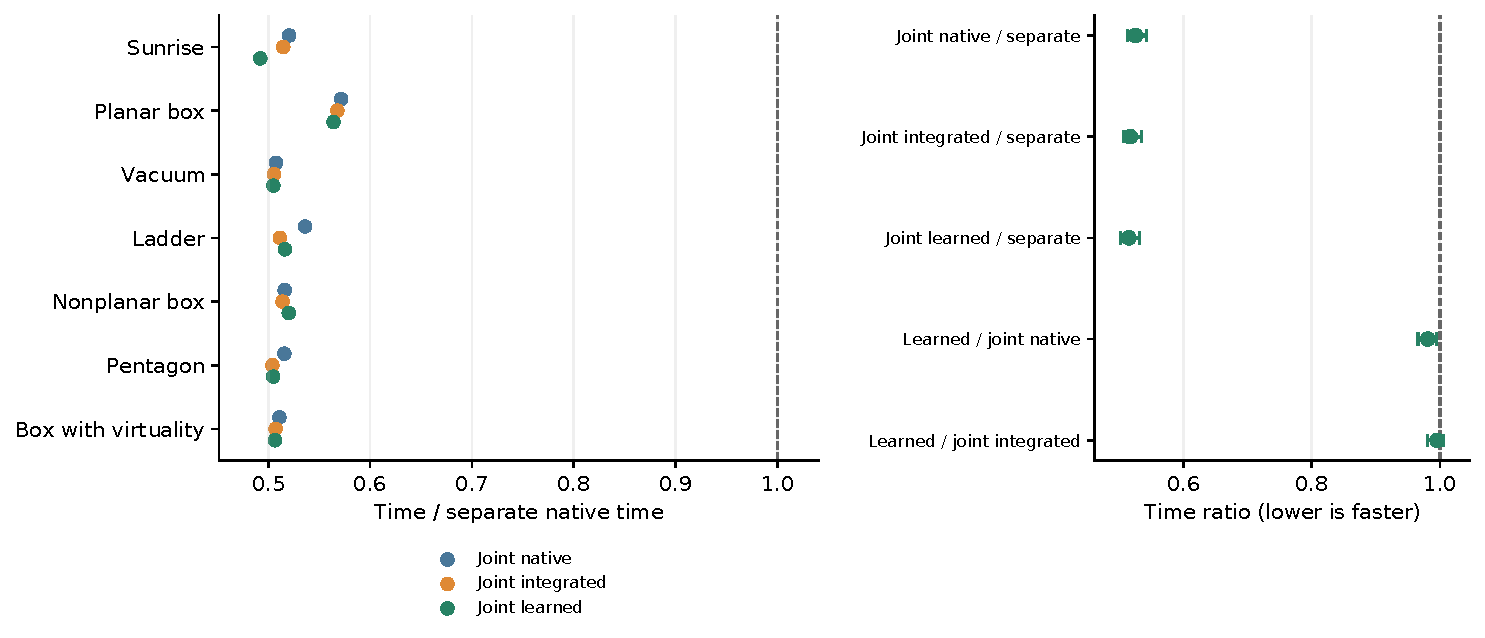
\includegraphics[width=\linewidth]{paper_figures/request_batching.pdf}
\caption{Combining compatible requests gives the main saving.
Left: ratios by graph relative to two separate native reductions.
Right: aggregate ratios and descriptive intervals. Comparing learned
choices with joint integrated native choices gives no reliable extra
saving. The panels retain the equal-time reference.}
\label{fig:joint}
\end{figure}

\FloatBarrier

The joint comparison reuses the main test's reserved parameter points, so it provides an additional comparison on that population. Its saving requires requests that can share one calculation. Transfer to new graph structures, isolated arbitrary integrals, and general scattering beyond three loops remains outside this result. The next study returns to individual batches and tests whether separate models and a wider set of seed strategies give a measurable gain.
